\documentclass{standalone}
\usepackage{tikz}
\begin{document}
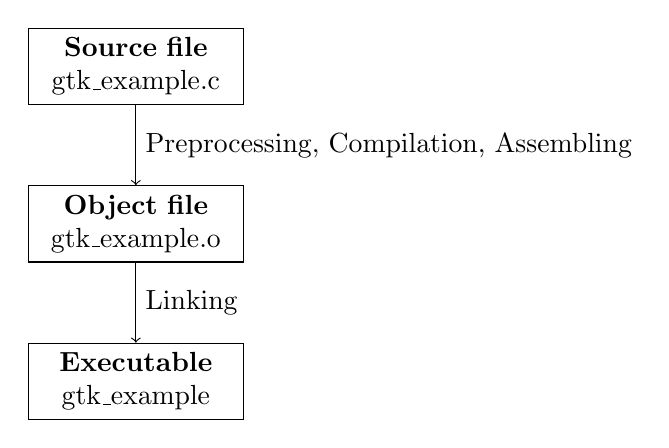
\begin{tikzpicture}[
    file/.style={draw,text width=2.5cm,align=center},
    arrow/.style={->,auto},
    node distance=2cm
  ]
  \node [file] (A) {\textbf{Source file}\\gtk\_example.c};
  \node [file,below of=A] (B) {\textbf{Object file}\\gtk\_example.o};
  \node [file,below of=B] (C) {\textbf{Executable}\\gtk\_example};
  \draw [arrow] (A) -- node {Preprocessing, Compilation, Assembling} (B);
  \draw [arrow] (B) -- node {Linking} (C);
\end{tikzpicture}
\end{document}
